\documentclass[11pt]{article}
\usepackage[a4paper,margin=25mm]{geometry}
\usepackage[T1]{fontenc}
\usepackage{lmodern}
\usepackage{booktabs}
\usepackage{amsmath}
\usepackage{graphicx}
\usepackage{hyperref}
\usepackage{xcolor}
\usepackage{listings}
\lstset{basicstyle=\ttfamily\small, columns=fullflexible, keepspaces=true,
  breaklines=true, frame=single, framerule=0.3pt, rulecolor=\color{gray}}
\newcommand{\code}[1]{\texttt{#1}}
\newcommand{\us}{\textmu s}

\title{\code{selection.py}: the event selection, step by step on one event}
\author{BGOTSCAN}
\date{2026-10-14}

\begin{document}
\maketitle

\section{Purpose}

Most recorded events are dark-count coincidences with no scintillation
pulse (see \code{runinfo\_doc.tex}); of the real events, some have their
pulse start before the record because the trigger fired late. The
selection must find the pulse, measure its charge, and classify the event
as empty, real, tail or pile-up. This script is the prototype of that
selection: it processes one event at a time, in twelve steps, and at each
step prints the numbers it computed and shows one figure, so that every
definition can be judged on real events before it is frozen in the Julia
pass (\code{JScan}). The definitions below are the ones the pass will
implement; this document is their reference.

It is a Python script in \code{src/py/}; it reads one event of the raw
HDF5 file with h5py and reuses the run lookup and the moving average of
\code{wfview.py}.

\section{Usage}

\begin{lstlisting}
python3 src/py/selection.py RUN [options]
\end{lstlisting}

Interactive: after each step the script waits on the terminal; Enter goes
to the next step, \code{n} abandons the event and starts the next one (for
instance once a maximum at the first sample has shown the event to be a
tail), \code{q} quits. At step~12 a number typed at the prompt redoes the
step with that zero-suppression threshold. The figure of the step stays open until
the next one. With \code{--save} there is no prompt: all steps run and
every figure is saved.

\begin{center}
\begin{tabular}{l l p{76mm}}
\toprule
option & default & meaning \\
\midrule
\code{--data DIR} & the data directory & as in \code{wfview.py} \\
\code{--events SPEC} & \code{0} & events to process: \code{a-b} or \code{a,b,c}, 0-based \\
\code{--cm METHOD} & \code{interp} & common-mode estimate used in step~5: \code{interp}, \code{median}, \code{none} \\
\code{--edge E} & 32 & samples averaged at each end of $W$ for the line of step~4 \\
\code{--baseline W} & \code{end} & baseline window of the sum: \code{end} of the record or \code{pre}-trigger \\
\code{--baseline-window N} & 250 & length of that window in samples (capped at the pre-trigger length for \code{pre}) \\
\code{--smooth N} & 64 & moving-average width of the pulse search, in samples \\
\code{--window A,B} & \code{1000,4000} & charge window: from $A$~ns before to $B$~ns after the smoothed maximum \\
\code{--nsigma K} & 5 & significance threshold used by the charge cut, the multiplicity and the pile-up search \\
\code{--zs k} & 3 & zero-suppression threshold of step~12, in units of the per-channel charge noise; can be changed at the prompt of that step \\
\code{--from-step N} & 1 & start at this step (earlier steps are computed silently) \\
\code{--save NAME} & off & no prompts; figures saved as \code{src/py/plots/NAME\_evE\_sN.png} \\
\code{--dump FILE} & off & write per event $t_{\max}$, $H$, $B$, $\sigma_1$, the charge and control windows, the 64 charges $q_c$ and the sum $S$ to a JSON file (reference for the tests of the Julia pass) \\
\bottomrule
\end{tabular}
\end{center}

\section{Notation}

$w_{c,i}$ is the raw ADC value of channel $c$ at sample $i$ ($i = 0 \dots
n_s-1$, $n_s = 3000$, $\Delta t = 8$~ns); $b_c$ the WebDump baseline of the
channel (attribute \code{baselines}); $x_{c,i} = w_{c,i} - b_c$. The time
axis is $t_i = (i - \code{pretrigger})\,\Delta t$ as in \code{wfview}. The
channels present are those of the dataset \code{channels}; $n_c$ is their
number (64). All rms values are standard deviations about the mean of the
window in question.

\section{The steps}

\subsection{Step 1: read the event}

Text: run, event index, \code{trigger\_id}, \code{timestamp\_ns}, the
interval to the previous recorded event, the number of board triggers since
it (difference of \code{trigger\_id} modulo $2^{24}$), pre-trigger and
sampling. Figure: $x_{c,i}$ for the 64 channels on an $8\times8$ grid in
channel order, shared axes.

\subsection{Step 2: common-mode analysis}
\label{sec:cm}

The low-frequency baseline noise is coherent across channels. Its estimate
is one value per sample, the median across the 64 channels,
\[
  m_i = \operatorname{median}_c\, x_{c,i}.
\]
The median rather than the mean because the estimate must not contain
signal: the mean is pulled by every lit channel in proportion to its
amplitude (a 20-count pulse in 10 channels shifts it by 3 counts), while
the median, the 32nd of the 64 values, hardly moves until more than half
the channels carry signal. The residual of a channel is $r_{c,i} = x_{c,i}
- m_i$. Nothing is subtracted at this step; it only characterises $m$.

Text: the definition of $m$; its rms over the record; the rms of $x_c$
and of $r_c$ averaged over channels, and the coherent fraction $1 -
\langle\mathrm{rms}\,r_c\rangle^2 / \langle\mathrm{rms}\,x_c\rangle^2$;
the rms of $m$ after a moving average of 0.1, 1 and 10~\us{} (12, 125,
1250 samples). White noise in $m$ falls as the square root of the window;
what survives at 10~\us{} is the genuine slow wander, the part worth
subtracting. Figure: three panels, top to bottom: the plain sum $\sum_c
x_{c,i}$, the starting point; $m_i$; one channel (the first) before and
after subtracting $m$.

A caveat drives the next step: during a real pulse many channels are
positive, so even $m_i$ contains some signal, and subtracting it from all
64 channels multiplies that leak by 64 in the sum.

\subsection{Step 3: locate the pulse (provisional)}

A first pass to find where the pulse is, so that the next step can keep it
out of the common-mode estimate. $S^0_i = \sum_c (x_{c,i} - m_i)$, minus
its median over the baseline window of step~6; $\hat S^0$ its moving
average of width $N_{\rm sm}$ (\code{--smooth}); $i^0_{\max} = \arg\max_i
\hat S^0_i$. Subtracting $m$ shrinks the pulse but does not move its
maximum, which is all this pass is used for. The window
\[
  W = [\,i^0_{\max} - a,\; i^0_{\max} + b\,], \qquad a = A/\Delta t,\; b = B/\Delta t
\]
(\code{--window}, default 1000 and 4000~ns), clipped to the record, is the
charge window of step~8 around the provisional maximum.

Text: $t^0_{\max}$ and its height, $a$, $b$, $W$ in ns and in samples.
Figure: $S^0$, $\hat S^0$, the maximum, $W$ shaded.

\subsection{Step 4: interpolate $m$ across $W$}

$\tilde m$ is $m$ outside $W$ and, inside $W$, a straight line between
\[
  L = \text{mean of } m \text{ over the } e \text{ samples before } W, \qquad
  R = \text{mean of } m \text{ over the } e \text{ samples after } W,
\]
with $e = 32$ (\code{--edge}): for $i_1 \le i \le i_2$, the first and
last samples of $W$, $\tilde m_i = L + (R - L)(i - i_1)/(i_2 - i_1)$. The
ends are averaged because each $m_i$ carries about 0.6 counts of noise;
built into the line and subtracted from all 64 channels that would be
40 counts of offset in the sum over the whole window; 32 samples (256~ns)
divide it by 5.7 while being short against the time scale of the wander.
If $W$ touches an edge of the record the missing end is replaced by the
other. $\tilde m$ contains no signal inside $W$ because it is built only
from samples outside the pulse; the price is that any wander faster than
the window length is left in across $W$.

Text: $L$, $R$, the sample ranges they come from, and the jump $R - L$ per
channel and times 64 in the sum. Figure: two panels, $m$ and $\tilde m$
over the whole record and zoomed around $W$, with $W$ and the two end
regions shaded.

\subsection{Step 5: subtract and sum}

The corrected channel is $y_{c,i} = x_{c,i} - \tilde m_i$ and the summed
waveform $S_i = \sum_c y_{c,i}$. For comparison the same is done with
$\tilde m = m$ (\code{median}: no protection of the pulse) and $\tilde m =
0$ (\code{none}); not with the mean, which makes the sum identically
zero.

Text: for each of the three estimates, the rms of $S$ in the control
window of step~8 and the charge in $W$, side by side, so that the loss of
signal and the gain in noise can be compared; the estimate chosen with
\code{--cm} is used from here on. Figure: $S$ with \code{none} and with
the chosen estimate, $W$ shaded.

\subsection{Step 6: baseline of the sum}

$B$ is the median of $S$ over the baseline window: the last $N$ samples
(\code{end}) or the first $N$ (\code{pre}, $N \le \code{pretrigger}$).
$\sigma_1$ is the rms of $S$ in that window, the per-sample noise of the
sum. From here on $S$ means $S - B$.

Text: $B$, $\sigma_1$, and the levels of both windows and their
difference, which measures the slow drift left after step~5. Figure: $S$
with both windows shaded and both levels drawn.

\subsection{Step 7: pulse search}

$\hat S$ is the moving average of $S$ of width $N_{\rm sm}$ (edges use the
samples available, as in \code{wfview}). The pulse is at $i_{\max} =
\arg\max_i \hat S_i$, height $H = \hat S_{i_{\max}}$. The rising edge
$i_{\rm rise}$ is the last sample before $i_{\max}$ with $\hat S_i < H/2$;
if there is none, the pulse is above half its maximum from the first
sample and the event has no rising edge. $\sigma_N$ is the rms of $\hat S$
in the control window.

Text: $t_{\max}$, $H$, $H/\sigma_N$, $t_{\rm rise}$ or ``no rising edge''.
Figure: $S$ and $\hat S$, with $i_{\max}$ and $i_{\rm rise}$ marked.

\subsection{Step 8: charge}

The charge window is $[i_{\max} - a,\; i_{\max} + b]$, the same shape as
$W$ around the final maximum, clipped to the record; $n$ its number of
samples. The charge is
\[
  Q = \Delta t \sum_{i = i_{\max}-a}^{i_{\max}+b} S_i \quad (\text{ADC}\cdot\text{ns}).
\]
The control window has the same length and lies in the pulse-free part of
the record: the longer of $[0, i_{\max}-a)$ and $(i_{\max}+b, n_s)$, and
within it the $n$ samples farthest from the pulse; if that part is shorter
than $n$ the whole of it is used and the text says so. $Q_{\rm ctrl}$ is
the same sum over the control window. The white-noise expectation for the
width of $Q$ is $\sigma_Q = \sigma_1 \sqrt{n}\,\Delta t$.

Text: $Q$, $Q_{\rm ctrl}$, $\sigma_Q$, $Q/\sigma_Q$ and $Q_{\rm
ctrl}/\sigma_Q$. Figure: $S$ with the two windows shaded.

\subsection{Step 9: multiplicity}

Per channel, the baseline $B_c$ is the median of $y_c$ over the baseline
window and the charge $q_c = \Delta t \sum_{\rm window} (y_{c,i} - B_c)$.
The same charge over the control window, $q_c^{\rm ctrl}$, has no signal;
its rms over the 64 channels, $\sigma_q$, is the per-channel charge noise,
one value for all channels, and it includes whatever slow per-channel
drift there is between the baseline window and the rest of the record
(the white-noise expectation $\langle\mathrm{rms}(y_c)_{\rm
ctrl}\rangle\sqrt{n}\,\Delta t$ is printed for comparison; it is smaller
when there is drift). The significance is $z_c = q_c / \sigma_q$ and the
multiplicity $M = \#\{c : z_c > K\}$.

Text: $\sigma_q$ and its white-noise expectation, $M$, the charge of the
channels above threshold next to $Q$, and their list. Figure: $8\times8$
map of $z_c$ in channel order.

\subsection{Step 10: verdict}

The pile-up search looks for a second pulse: the maximum $P_2$ of $\hat S$
outside the charge window, at $i_2$, and the valley $V = \min \hat S$
between $i_{\max}$ and $i_2$. It is a pile-up if $P_2 > K\sigma_N$ and
$P_2 - V > K\sigma_N$: the second maximum is significant and the sum
drops significantly between the two. Without the valley condition the
tail or the smoothed rise of the main pulse, just outside the charge
window, passes as a second pulse in most events. The verdict is:
\begin{itemize}
\item \emph{empty}: $Q < K \sigma_Q$;
\item \emph{real}: $Q \ge K \sigma_Q$ and a rising edge was found;
\item \emph{tail}: $Q \ge K \sigma_Q$ and no rising edge: the pulse started before the record and only its tail was recorded;
\item plus the flag \emph{pile-up} if a second maximum was found.
\end{itemize}
Text only: the verdict with the numbers it rests on ($Q/\sigma_Q$, the
rising edge, $M$, $P_2$ and its position, $V$, the prominence $P_2 - V$),
one line. Then the next event.

\subsection{Step 11: zero suppression, charge kept versus threshold}

Writing the 64 corrected waveforms of every event would quadruple the data
volume, while the light of an event sits in a dozen channels. Zero
suppression keeps, event by event, the channels whose charge is
significant: with $q_c$ and $\sigma_q$ from step~9, channel $c$ is kept if
$z_c = q_c/\sigma_q > k$. The cost is the charge of the dropped channels.
With $Q_{\rm all} = \sum_c q_c$ over the 64 channels and $Q_{\rm kept}(k)$
the sum over the kept ones, the fraction kept is $Q_{\rm kept}/Q_{\rm
all}$. Dropped channels carry small charges of either sign, so the
fraction can exceed one.

Text: for $k = 0, 1, 2, 3, 5, 8$, the number of channels kept, $Q_{\rm
kept}$ and the fraction kept, one line per $k$. Figure: two panels over
the channel rank (channels sorted by decreasing $z_c$): the bars of
$z_c$ with the thresholds drawn, and the cumulative fraction of $Q_{\rm
all}$ as more channels are included.

\subsection{Step 12: zero suppression, the kept channels}

The event at one threshold, $k$ from \code{--zs} or typed at the prompt.
Text: $k$, the kept channels, $Q_{\rm kept}/Q_{\rm all}$, and the rms in
the control window of the sum of the kept channels against that of the
full sum (dropping noise channels lowers the noise of the sum). Figure:
the $8\times8$ grid with only the kept channels drawn, and the sum of the
kept channels over the full sum, to see that the pulse shape is
preserved. A number at the prompt redoes the step with that $k$; Enter
accepts and goes to the next event. The waveforms kept are float32.

\section{A walk through one event}

Event 1 of \code{197K\_39V\_th20}, produced with
\begin{lstlisting}
python3 src/py/selection.py 197K_39V_th20 --events 1 --save walk
\end{lstlisting}
and the figures copied to \code{docs/figs/sel\_197K\_ev1\_sN.png}. For
each step, the text the script printed and what to look at in the figure.

\paragraph{Step 1: read.}
\begin{lstlisting}
step 1: 197K_39V_th20 event 1: trigger_id 3055990, timestamp 7515872841.232 us,
  23.070 ms and 149 board triggers after event 0; pre-trigger 200 samples,
  8 ns/sample, 3000 samples
\end{lstlisting}
The 149 board triggers in 23~ms since the previous recorded event are the
readout gap of \code{runinfo\_doc.tex}. In the figure, a pulse is visible
by eye in channels 48 to 53, 11 and 12, as a bump of 10 to 20 counts
decaying over a microsecond at $t = 0$; the other channels are flat
noise of 4 counts rms with isolated single-photoelectron spikes.

\begin{center}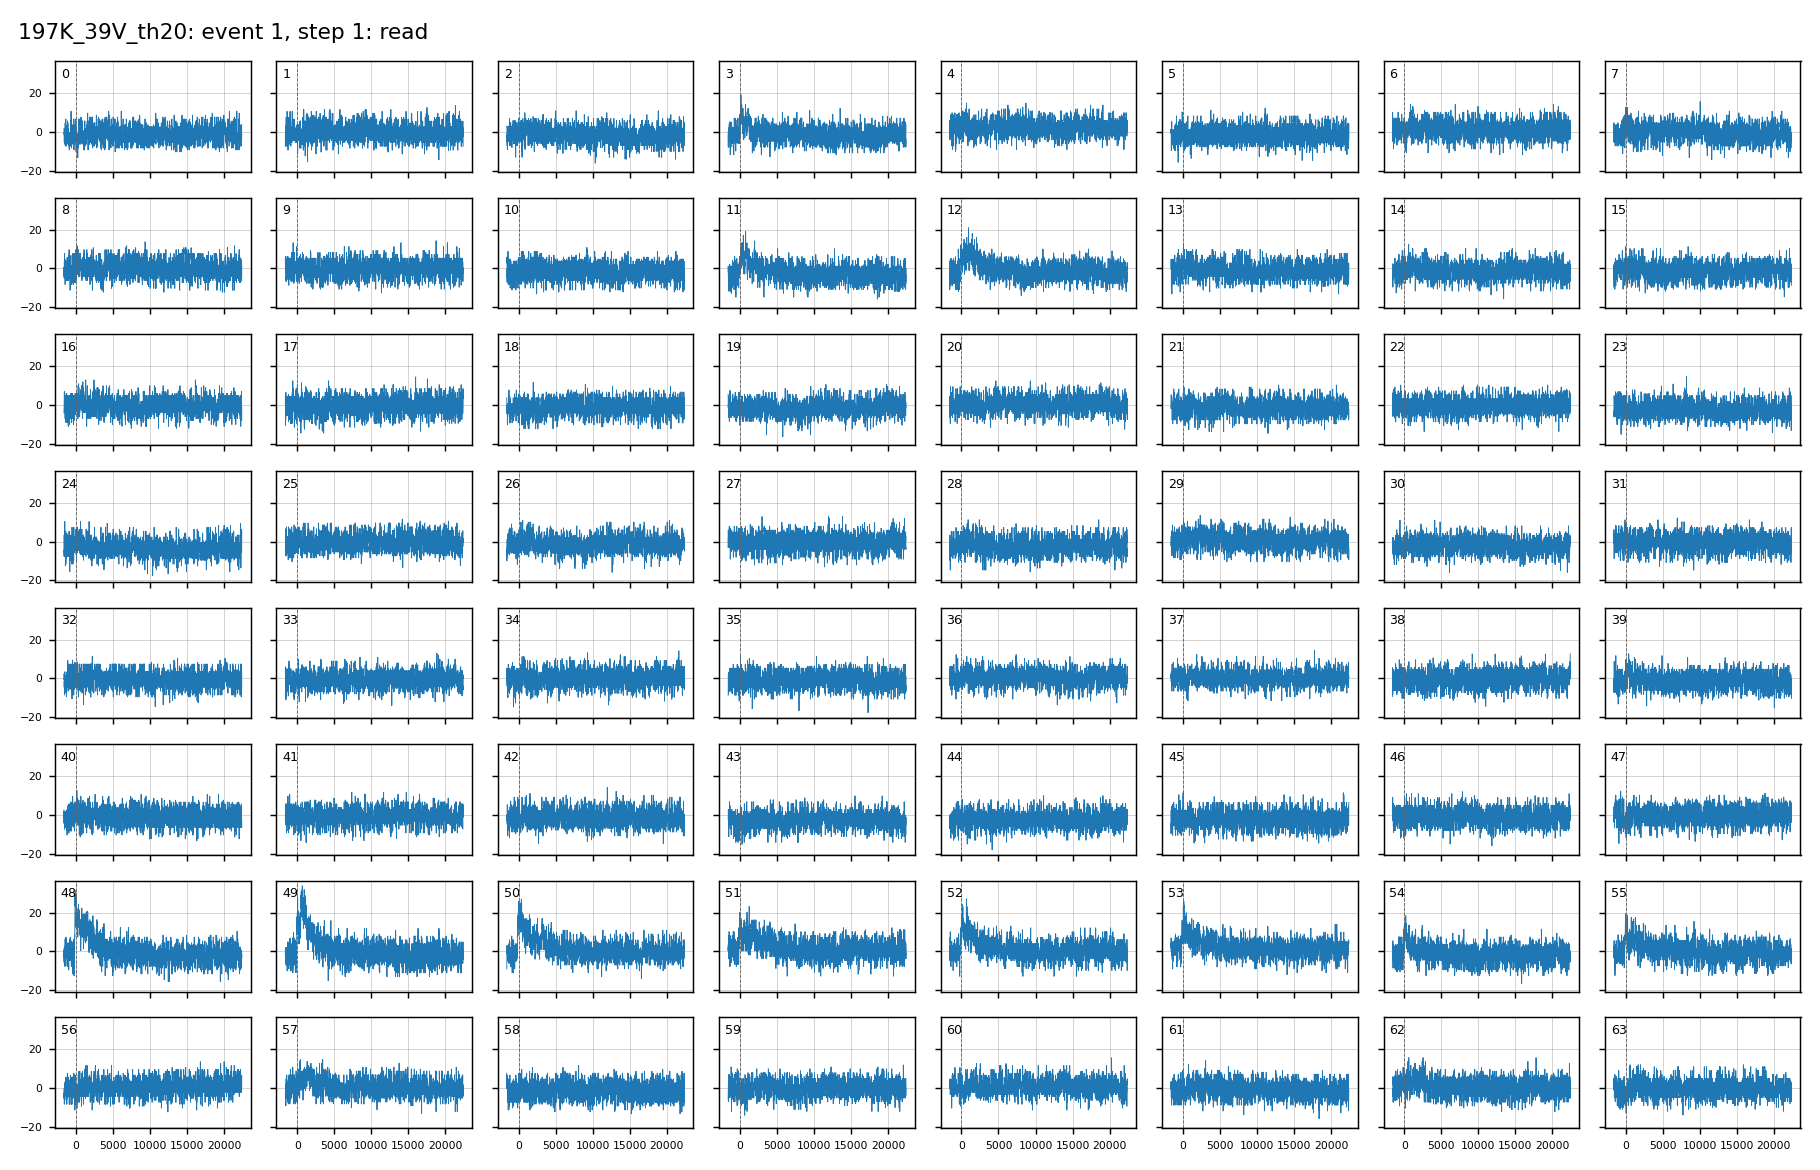
\includegraphics[width=\textwidth]{figs/sel_197K_ev1_s1.png}\end{center}

\paragraph{Step 2: common-mode analysis.}
\begin{lstlisting}
step 2: m[i] = median over the 64 channels of x[c,i], one value per sample:
  rms 0.78 ADC; channel rms 4.03, residual (channel minus m) rms 3.97,
  coherent fraction 0.03; rms of m after 0.1 / 1 / 10 us smoothing: 0.49 / 0.43 / 0.28
\end{lstlisting}
Top: the plain sum, the pulse of 200 counts over 35 counts of noise, on
a baseline that sits 50 counts below zero over most of the record. Middle:
$m$; it is below one count, but it rises by 1.5 counts during the pulse,
following the shape of the sum: that is signal entering the median.
Bottom: one channel before and after subtracting $m$, indistinguishable,
as the coherent fraction of 3\% says.

\begin{center}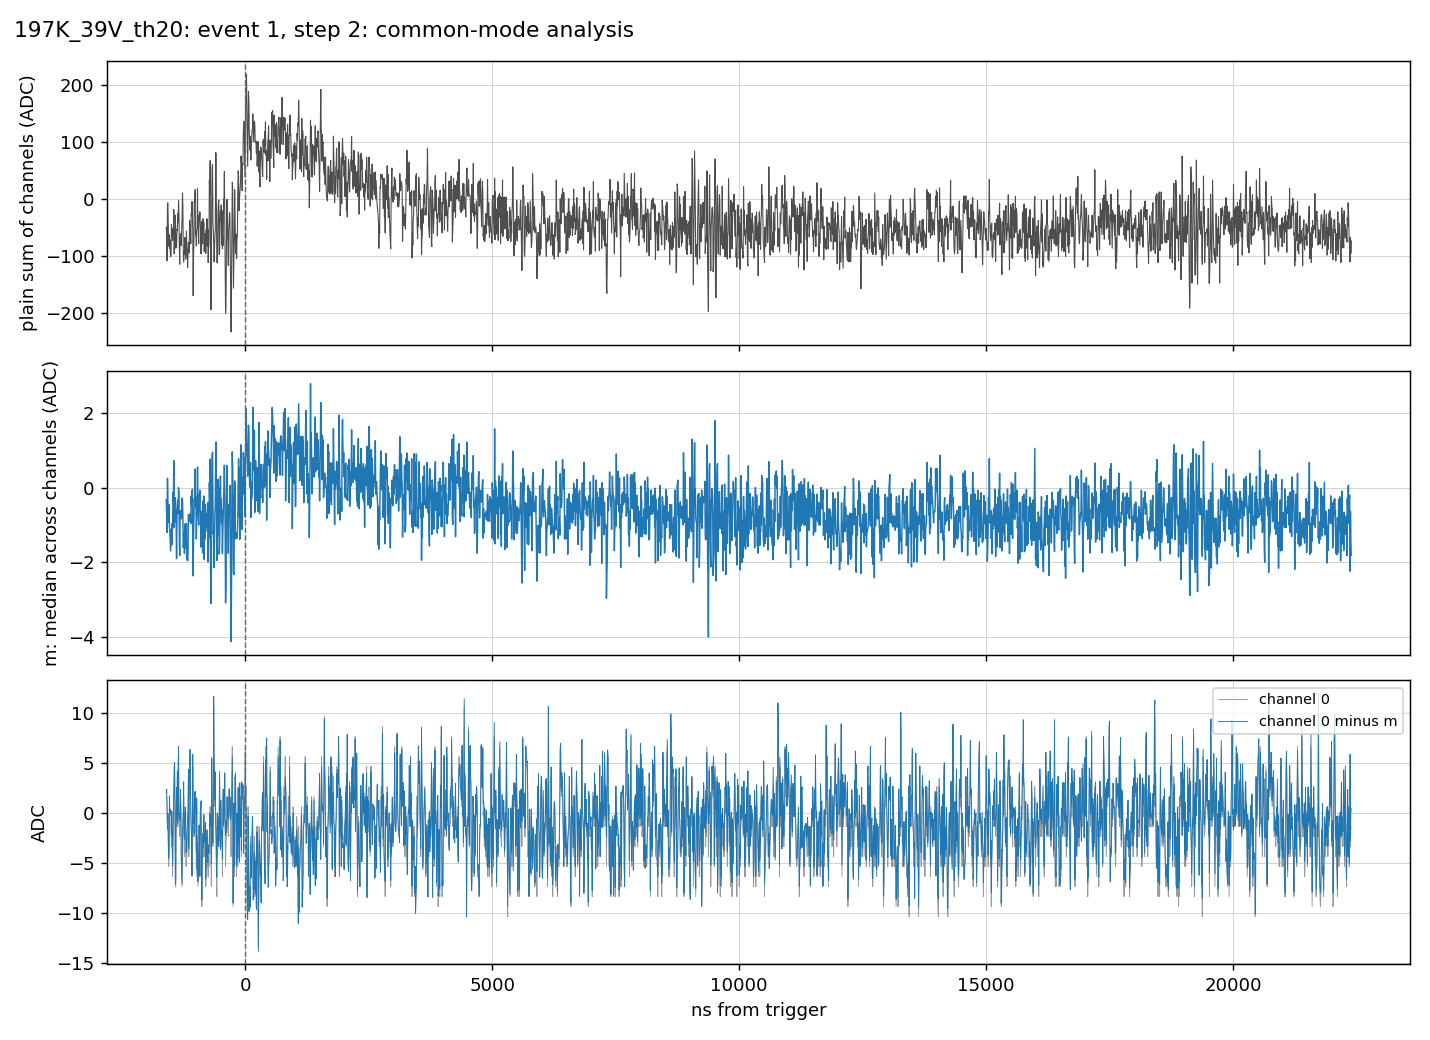
\includegraphics[width=\textwidth]{figs/sel_197K_ev1_s2.png}\end{center}

\paragraph{Step 3: locate the pulse.}
\begin{lstlisting}
step 3: S0 = sum over channels of (x - m), moving average over 64 samples:
  maximum 72.1 ADC at 176 ns (sample 222); W = [imax - a, imax + b] with
  a = 125, b = 500 samples: [-824, 4176] ns = samples [97, 722], 626 samples
\end{lstlisting}
The pulse found on the median-subtracted sum, shrunk to 72 counts by the
leak of step~2 but at the right place. $W$ is the shaded band.

\begin{center}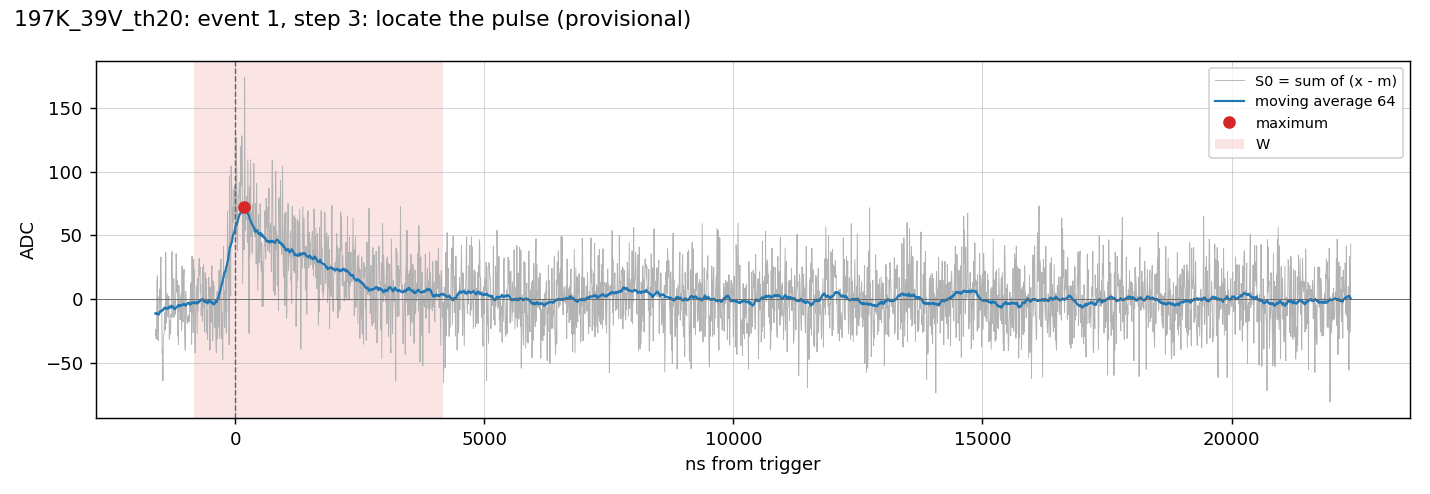
\includegraphics[width=\textwidth]{figs/sel_197K_ev1_s3.png}\end{center}

\paragraph{Step 4: interpolate $m$ across $W$.}
\begin{lstlisting}
step 4: L = mean of m over 32 samples before W, samples [65, 96]: -0.69 ADC;
  R = mean over 32 samples after W, samples [723, 754]: 0.04 ADC; mt = m outside W,
  straight line from L to R inside W; jump R - L = +0.73 ADC per channel = +47 ADC in the sum
\end{lstlisting}
The bottom panel is the one to look at: inside $W$ the median (grey)
carries the pulse, the line (blue) passes underneath from $L$ to $R$. The
jump of 0.7 counts between the two ends is the slow wander across the
window, 47 counts in the sum.

\begin{center}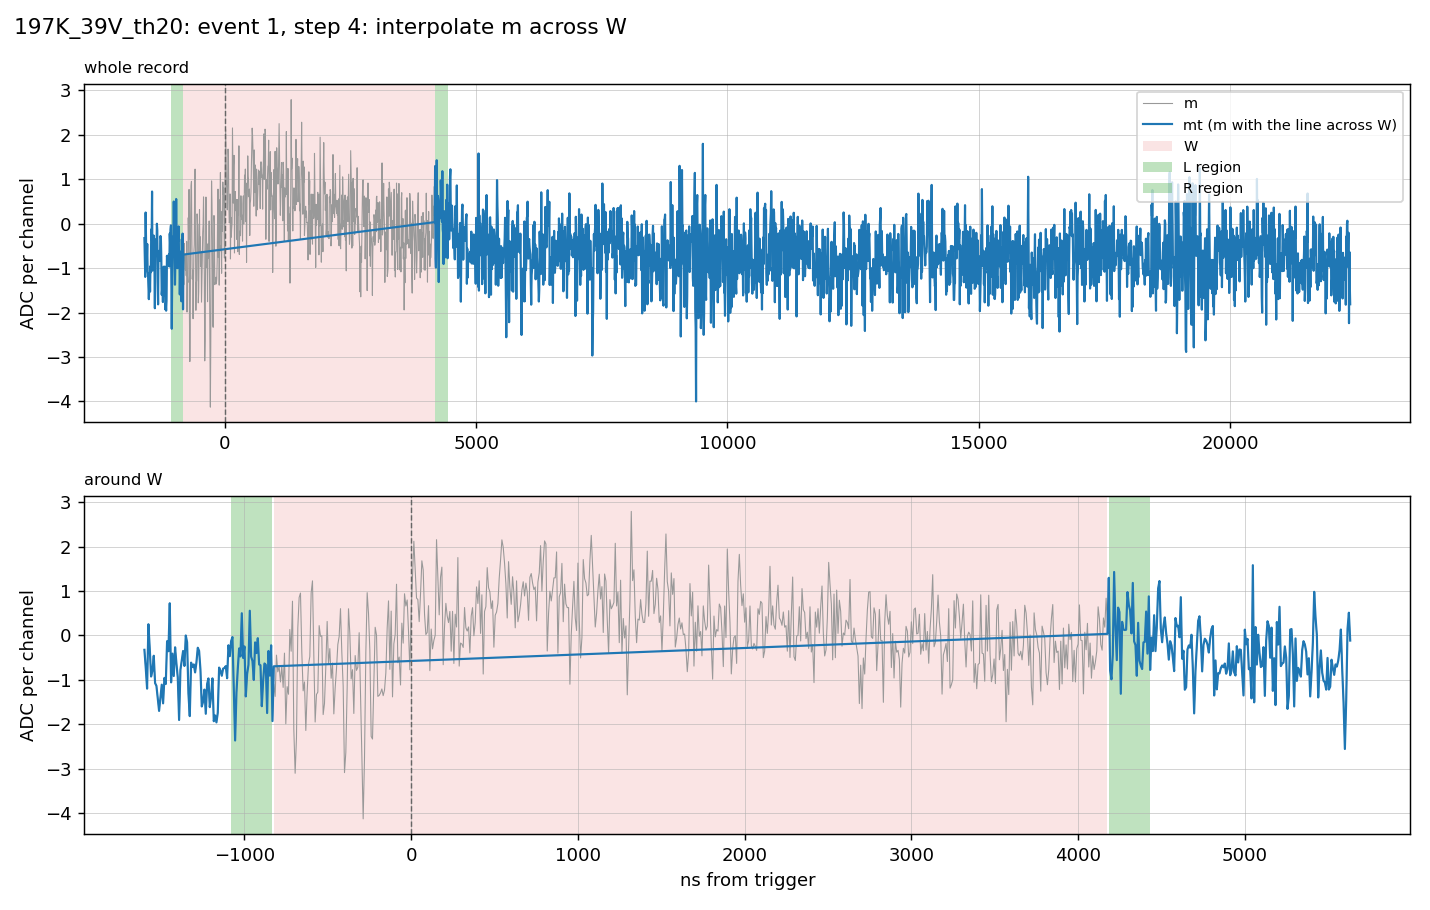
\includegraphics[width=\textwidth]{figs/sel_197K_ev1_s4.png}\end{center}

\paragraph{Step 5: subtract and sum.}
\begin{lstlisting}
step 5: y = x - estimate for every channel, S = sum of y, minus its median over
  the baseline window; per estimate, rms of S in the control window and charge in W:
        median  control rms    22.8 ADC   charge    1.166e+05 ADC ns
        interp  control rms    22.8 ADC   charge    2.591e+05 ADC ns
        none    control rms    35.0 ADC   charge    4.186e+05 ADC ns
        using interp
\end{lstlisting}
The three lines are the point of the method: \code{median} and
\code{interp} have the same noise in the control window, 23 counts
against 35 without subtraction, but \code{median} keeps only 45\% of the
charge that \code{interp} keeps. The \code{none} charge is larger still
because it includes the wander across $W$ that \code{interp} removes.
Figure: the sum with no subtraction and with \code{interp}.

\begin{center}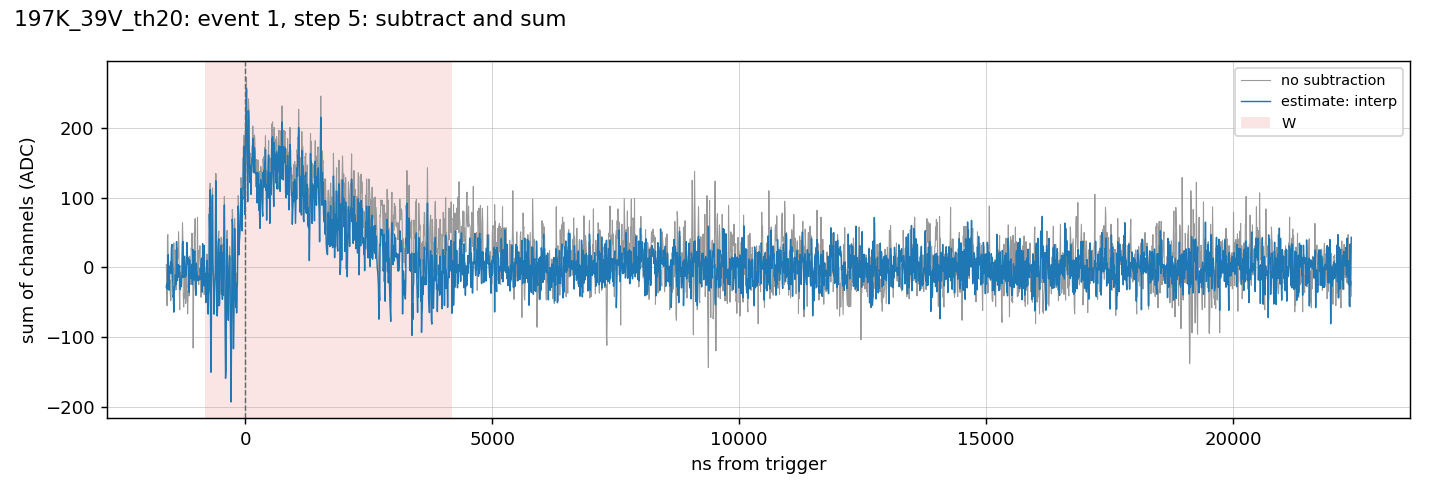
\includegraphics[width=\textwidth]{figs/sel_197K_ev1_s5.png}\end{center}

\paragraph{Step 6: baseline.}
\begin{lstlisting}
step 6: baseline (end, 250 samples) 0.0 ADC, per-sample rms 24.0; end-of-record
  level 0.0, pre-trigger level -10.4, difference +10.4
\end{lstlisting}
The baseline is taken from the end window, so its level is zero by
construction; the pre-trigger window, 1.6~\us{} earlier, sits 10 counts
lower, the residual slow drift over the record.

\begin{center}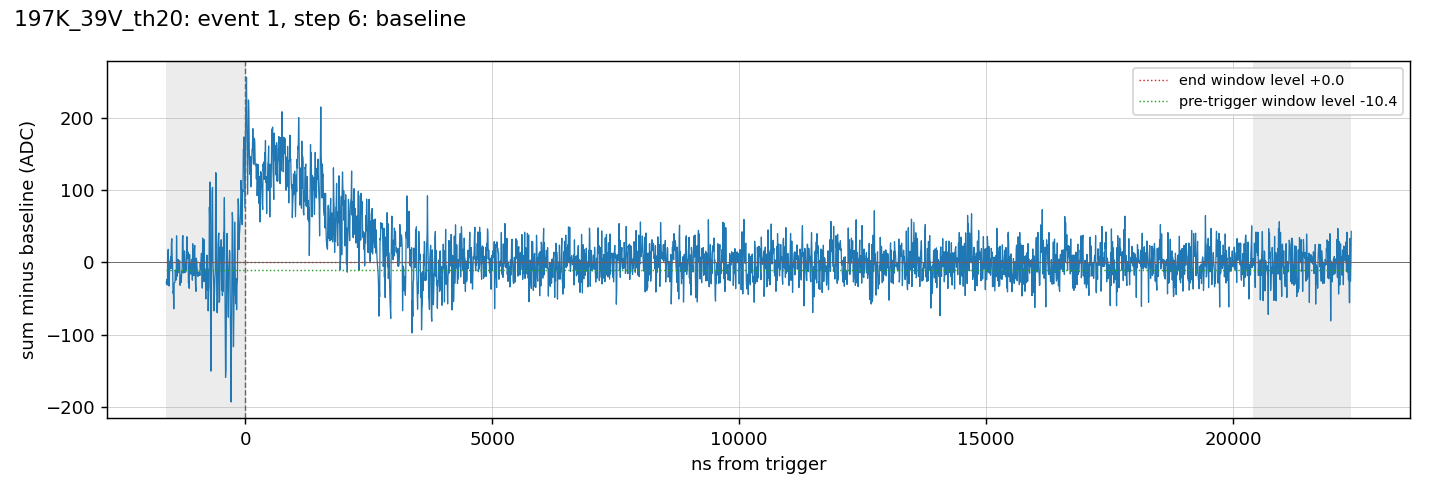
\includegraphics[width=\textwidth]{figs/sel_197K_ev1_s6.png}\end{center}

\paragraph{Step 7: pulse search.}
\begin{lstlisting}
step 7: smoothed (64 samples) maximum 138.3 ADC at 696 ns, 71.0 x control rms 1.9;
  rising edge (half maximum) at -88 ns
\end{lstlisting}
The moving average (blue) peaks at 138 counts, 71 times its noise; the
rising edge, where it crosses half maximum, is 88~ns before the trigger,
and the maximum 0.7~\us{} after it. This is the key figure for the class
of the event (next section).

\begin{center}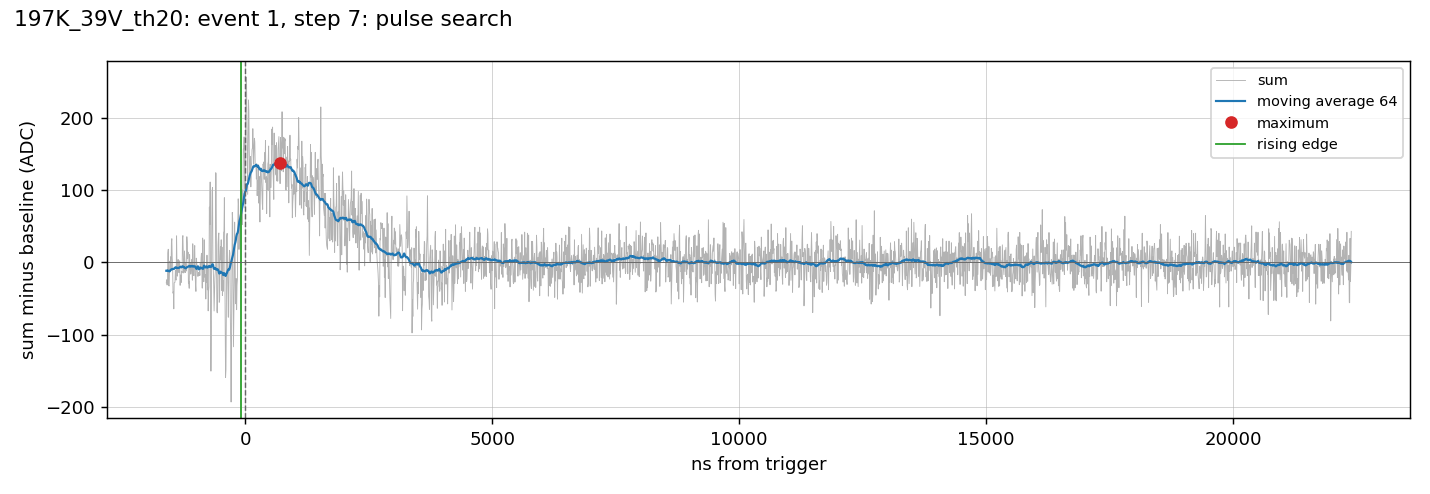
\includegraphics[width=\textwidth]{figs/sel_197K_ev1_s7.png}\end{center}

\paragraph{Step 8: charge.}
\begin{lstlisting}
step 8: charge window [-304, 4696] ns (626 samples): Q 2.648e+05 ADC ns; control
  window [17392, 22392] ns: -4469; white-noise width 4812; Q/width 55.0, control/width -0.9
\end{lstlisting}
The charge window (red) around the final maximum and the control window
(grey) at the end of the record. The control charge is $-0.9$ widths,
consistent with noise; the pulse charge is 55 widths.

\begin{center}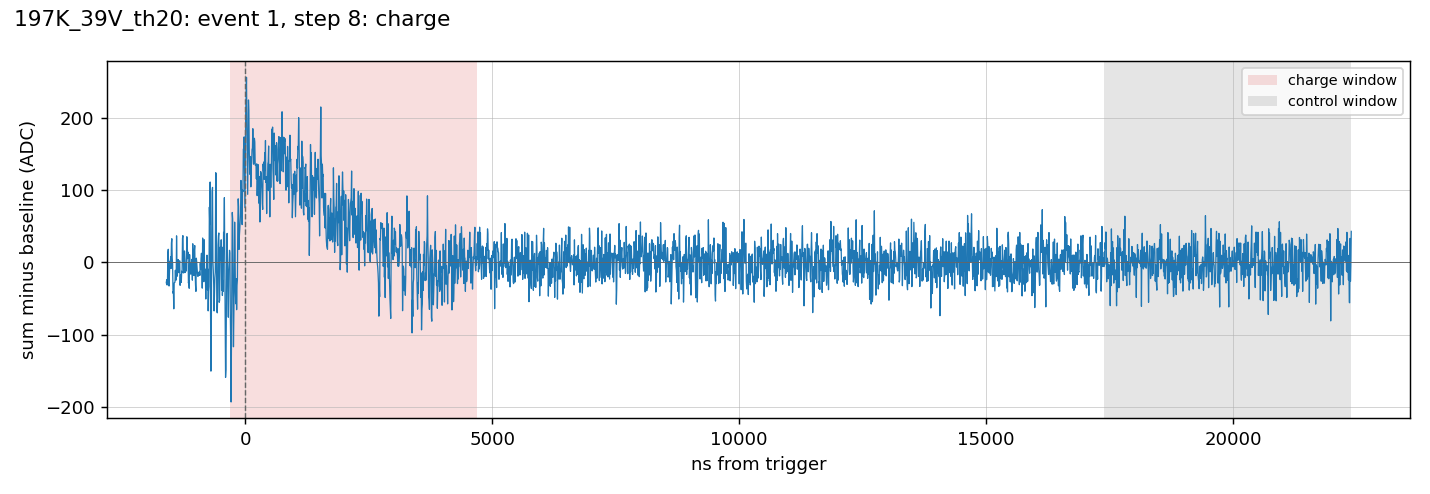
\includegraphics[width=\textwidth]{figs/sel_197K_ev1_s8.png}\end{center}

\paragraph{Step 9: multiplicity.}
\begin{lstlisting}
step 9: per-channel charge noise 2364 ADC ns from the control window (white-noise
  expectation 756.6); multiplicity 11 channels above 5 sigma, their charge 3.084e+05
  vs Q 2.648e+05; channels: [11, 12, 48, 49, 50, 51, 52, 53, 54, 55, 57]
\end{lstlisting}
The per-channel charge noise is three times the white-noise value, from
per-channel slow drift. Eleven channels are above 5 sigma: the row 48 to
55 and 11, 12, the same channels seen by eye in step~1. Their charge
exceeds $Q$ because the other 53 channels sum to a negative drift.

\begin{center}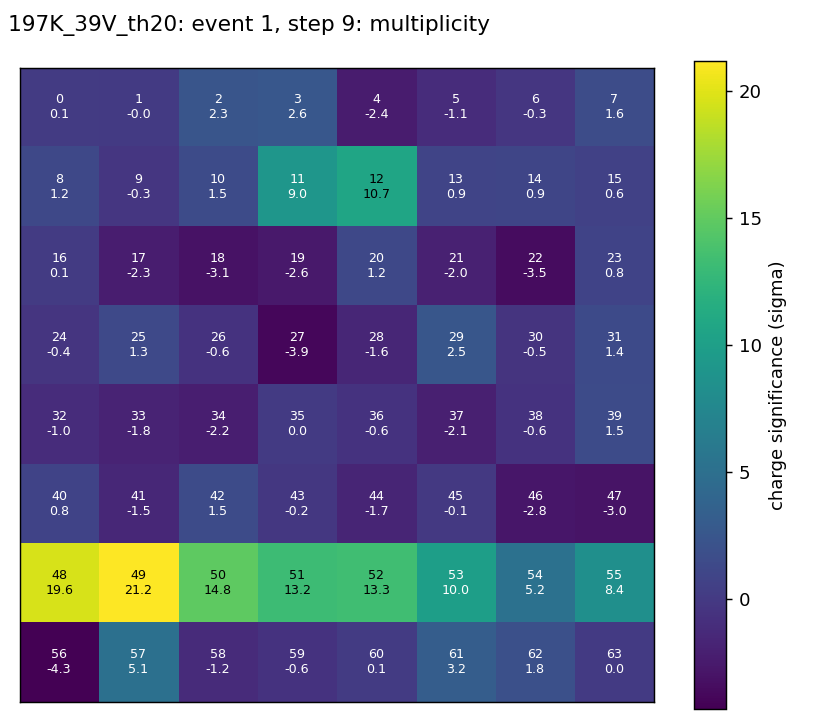
\includegraphics[width=0.6\textwidth]{figs/sel_197K_ev1_s9.png}\end{center}

\paragraph{Step 10: verdict.}
\begin{lstlisting}
step 10: REAL: Q/width 55.0 (cut 5), rising edge found, multiplicity 11; second maximum
  9.0 ADC at 7800 ns (4.6 x smoothed control rms), valley between the maxima -15.3 ADC,
  prominence 24.4 (12.5 x)
\end{lstlisting}
Charge above the cut and a rising edge: REAL. The second maximum outside
the window is 4.6 noise widths, below the cut of 5, so no pile-up.

\paragraph{Step 11: zero suppression, charge kept versus threshold.}
\begin{lstlisting}
step 11: zero suppression keeps channel c if q_c / sigma_q > k; Q_all = sum over 64
  channels 2.609e+05 ADC ns; per threshold k: channels kept, Q_kept, fraction kept
        k =   0   kept 34   Q_kept    3.749e+05   fraction  1.437
        k =   1   kept 24   Q_kept    3.646e+05   fraction  1.397
        k =   2   kept 15   Q_kept    3.336e+05   fraction  1.278
        k =   3   kept 12   Q_kept     3.16e+05   fraction  1.211
        k =   5   kept 11   Q_kept    3.084e+05   fraction  1.182
        k =   8   kept  9   Q_kept     2.84e+05   fraction  1.089
\end{lstlisting}
Top: nine channels above 8 sigma, then a long tail of small positive
values down to rank 30, and 30 channels with negative charge, down to
$-4$ sigma. Bottom: the cumulative charge rises past $Q_{\rm all}$ at
rank 9, peaks at 1.44 at rank 34 and comes back to 1 only when the
negative channels are added. The channels without light do not sum to
zero in this event: their drift over the charge window is net negative
and worth 30\% of $Q_{\rm all}$. Zero suppression removes that drift
along with the small positive tail, so $Q_{\rm kept}$ is larger than
$Q_{\rm all}$ for any $k$; which of the two is the better estimate of the
light is a question for the distributions over many events.

\begin{center}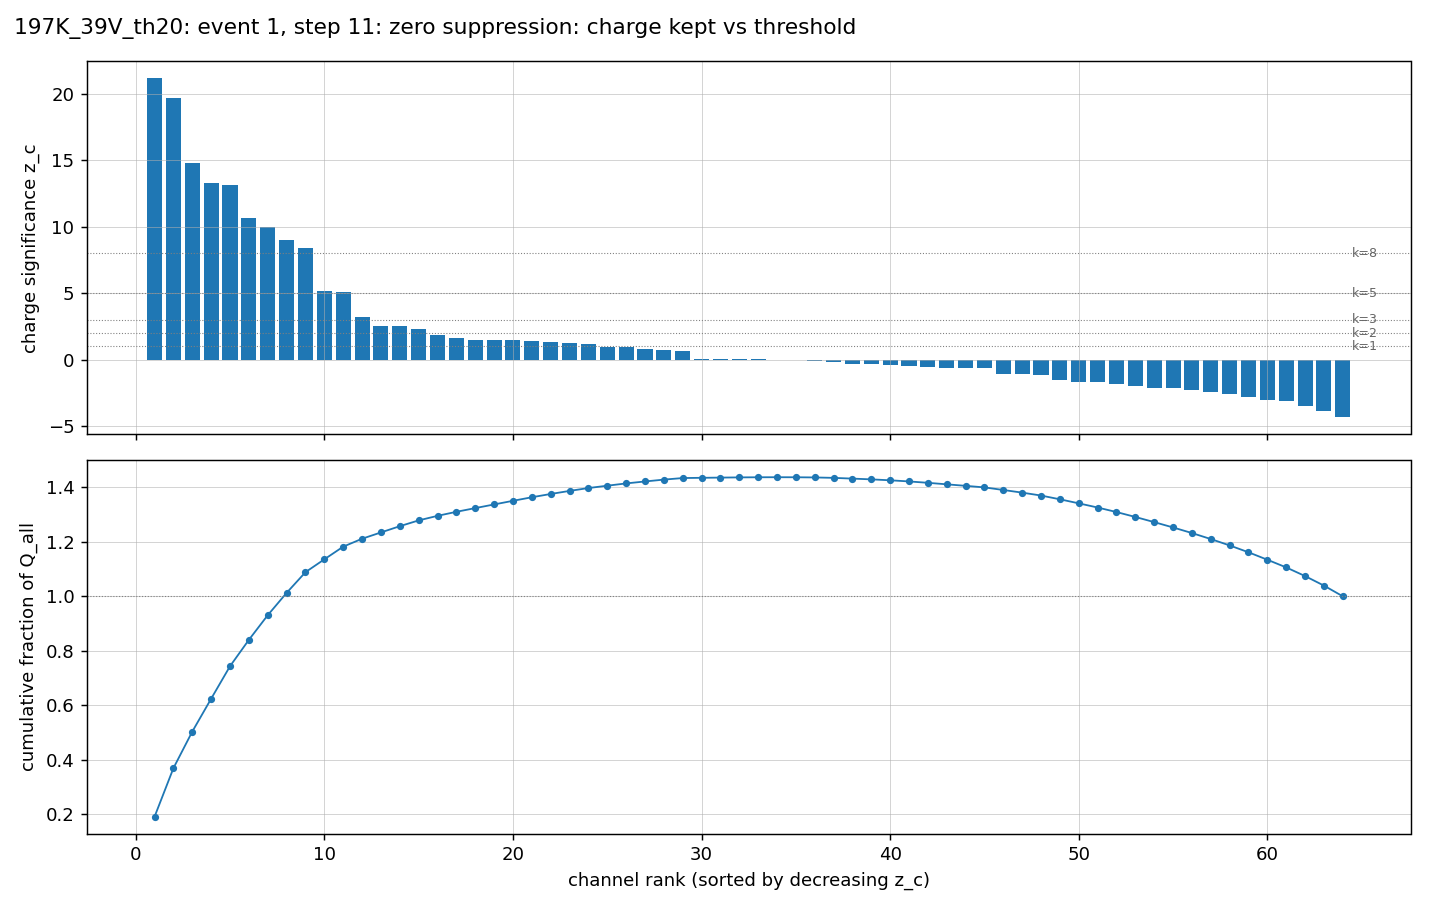
\includegraphics[width=\textwidth]{figs/sel_197K_ev1_s11.png}\end{center}

\paragraph{Step 12: zero suppression, the kept channels.}
\begin{lstlisting}
step 12: k = 3: 12 channels kept [11, 12, 48, 49, 50, 51, 52, 53, 54, 55, 57, 61];
  Q_kept/Q_all 1.211; control rms of the kept sum 12.4 ADC vs full sum 22.8
\end{lstlisting}
At $k = 3$ the twelve kept channels are the row 48 to 55 plus 11, 12, 57
and 61. The sum of the kept channels (blue, bottom panel) has the same
pulse as the full sum (grey) with half the noise: dropping 52 channels
drops their noise too. A number typed at the prompt redraws the figure
with that threshold.

\begin{center}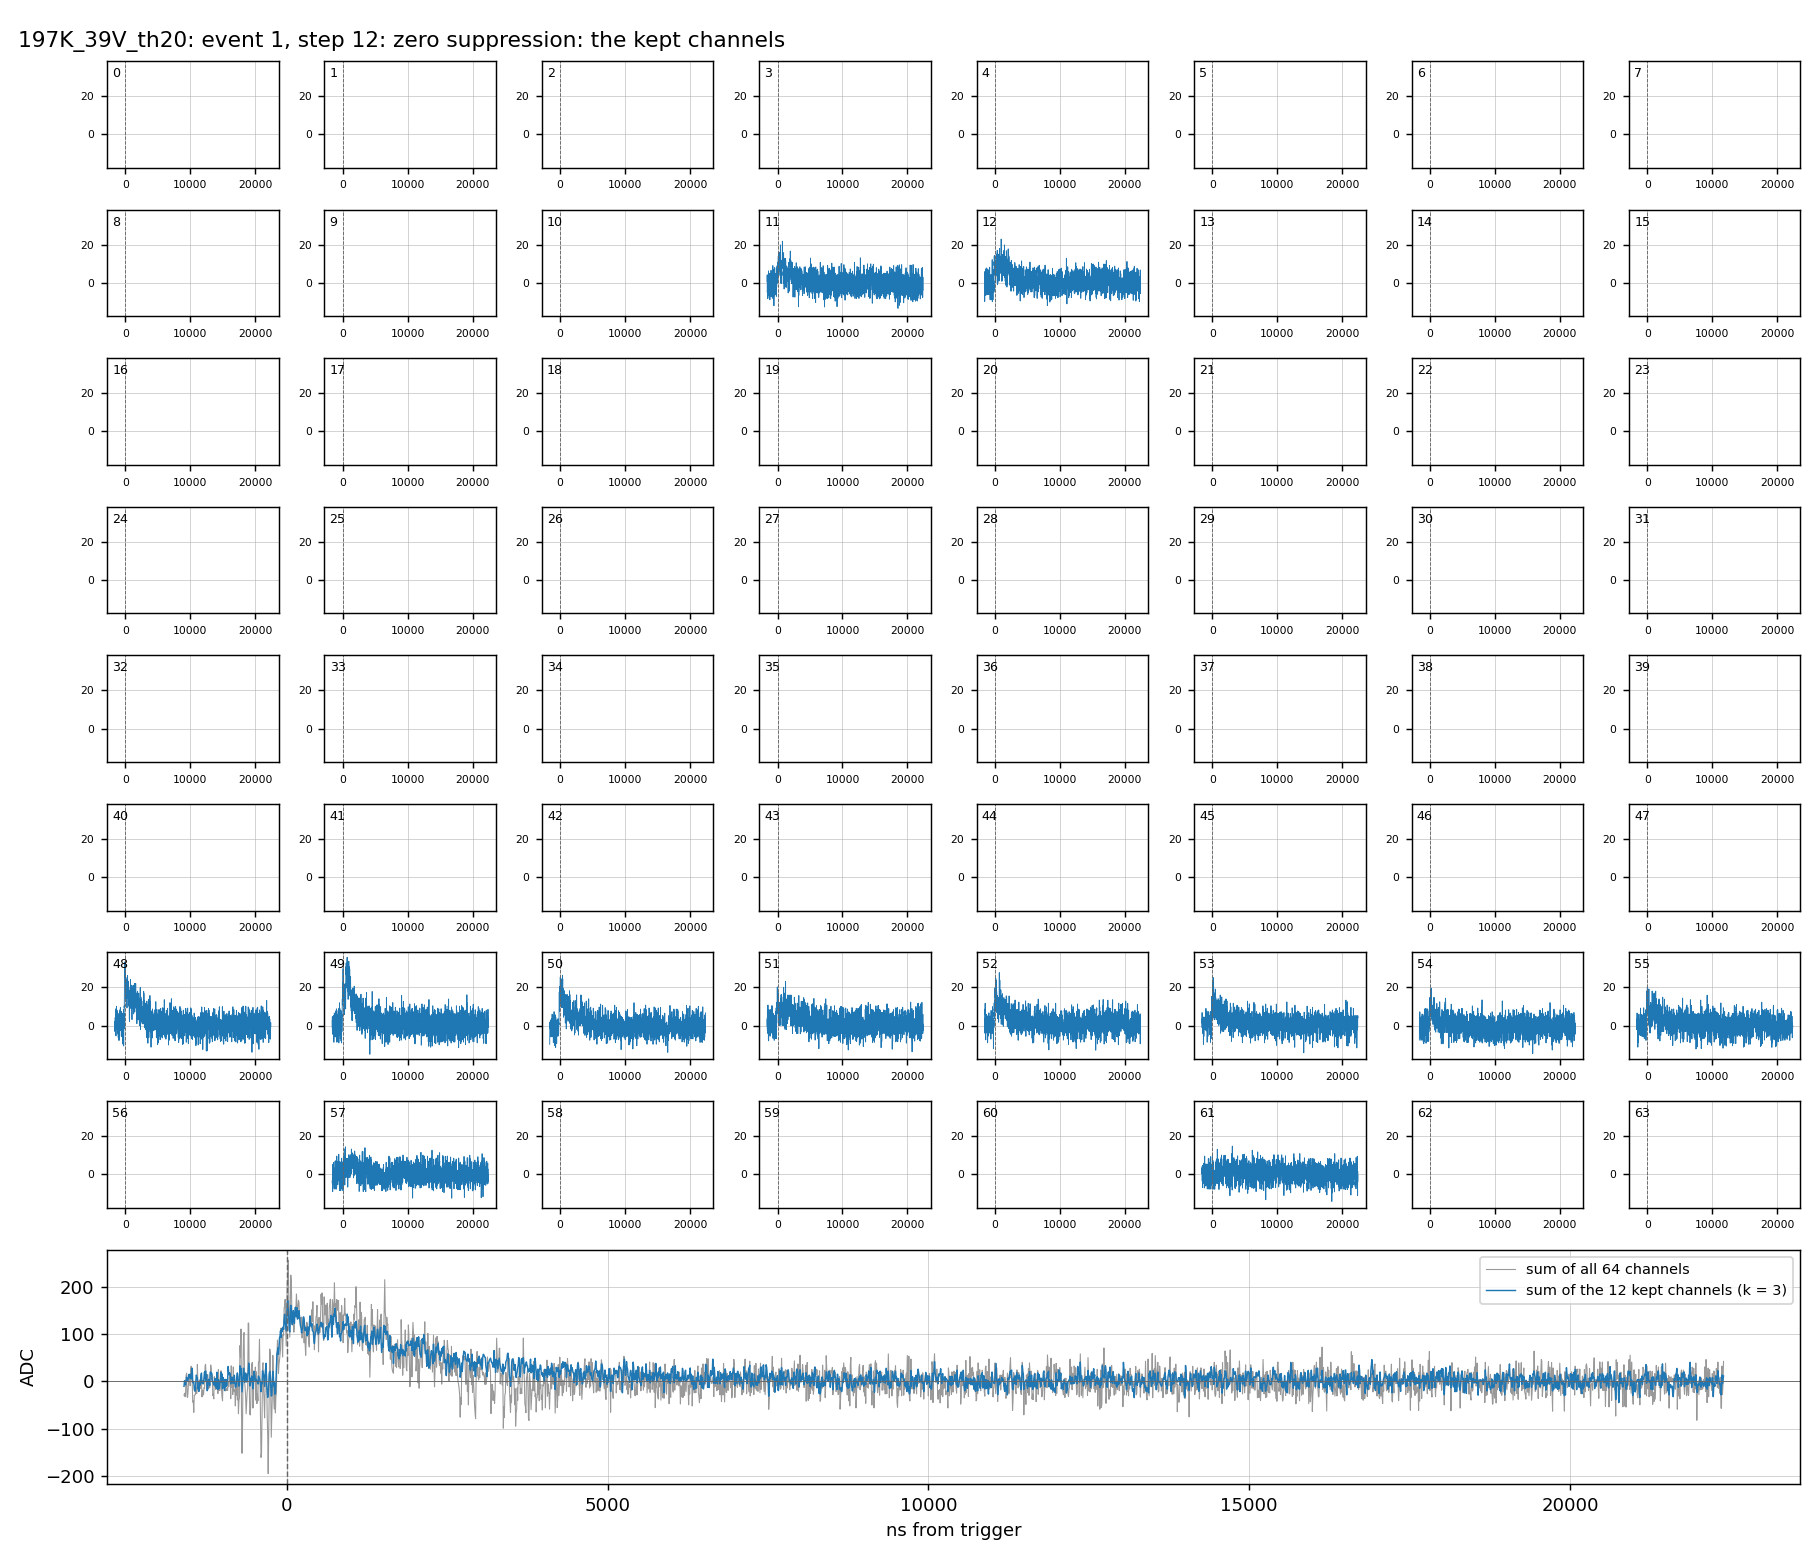
\includegraphics[width=\textwidth]{figs/sel_197K_ev1_s12.png}\end{center}

\section{Identifying the class}

The figure of step~7, the sum with its moving average, the maximum and
the rising edge, decides the class. Three events, one per class.

\paragraph{REAL: rising edge found, maximum after it.} Event 1 of
\code{197K\_39V\_th20} (above): the moving average is at the noise level
before the trigger, crosses half maximum at $-88$~ns and peaks at
$+0.7$~\us. The script prints ``rising edge (half maximum) at $-88$ ns''.

\paragraph{TAIL: no rising edge, maximum at the first sample.} Event 0
of \code{128K\_37V\_th19}:
\begin{lstlisting}
step 7: smoothed (64 samples) maximum 85.3 ADC at -1568 ns, 25.0 x control rms 3.4;
  no rising edge
step 10: TAIL: Q/width 34.6 (cut 5), no rising edge, multiplicity 10; ...
\end{lstlisting}
The sum is at its maximum at the start of the record and decays from
there: the pulse started before the record, more than 1.6~\us{} before
the trigger fired, and only its tail was recorded. The charge is
significant but incomplete.

\begin{center}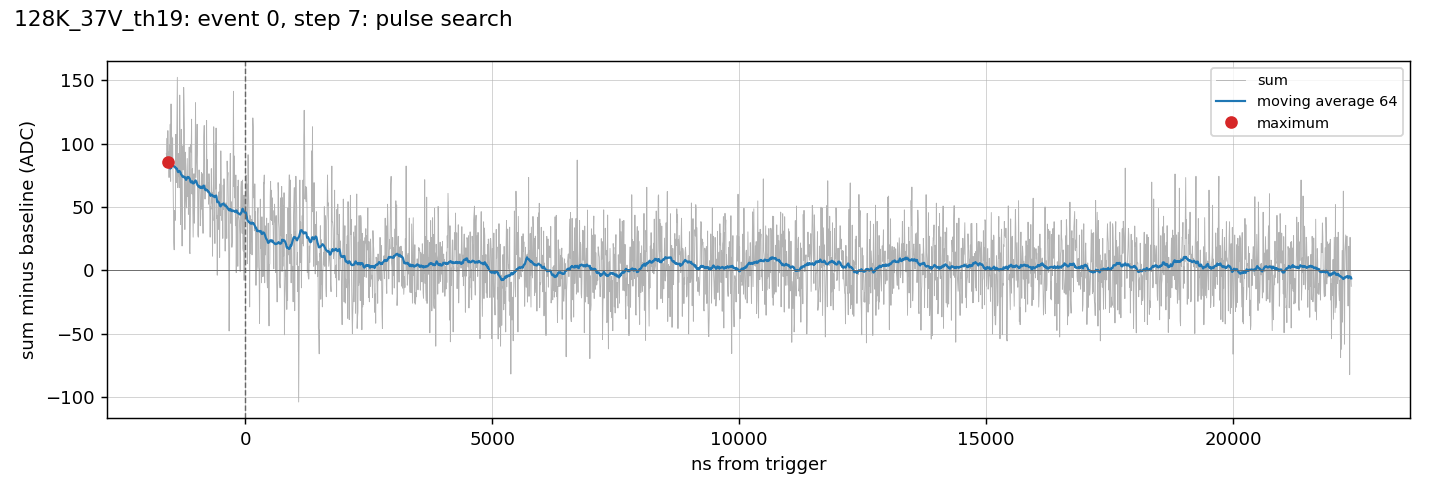
\includegraphics[width=\textwidth]{figs/sel_128K_ev0_s7_tail.png}\end{center}

\paragraph{PILE-UP: two maxima with a valley between them.} Event 18 of
\code{197K\_39V\_th20}:
\begin{lstlisting}
step 7: smoothed (64 samples) maximum 130.9 ADC at -344 ns, 50.5 x control rms 2.6;
  rising edge (half maximum) at -656 ns
step 10: REAL + PILE-UP: Q/width 83.6 (cut 5), rising edge found, multiplicity 9;
  second maximum 35.6 ADC at 12720 ns (13.7 x smoothed control rms), valley between
  the maxima -8.9 ADC, prominence 44.5 (17.2 x)
\end{lstlisting}
A second pulse at 12.7~\us{}, 14 noise widths high, with the sum back at
zero between the two. The valley condition matters: the tail of the main
pulse just outside the charge window is often above the threshold too,
but there is no valley between it and the maximum, so it is not a second
pulse.

\begin{center}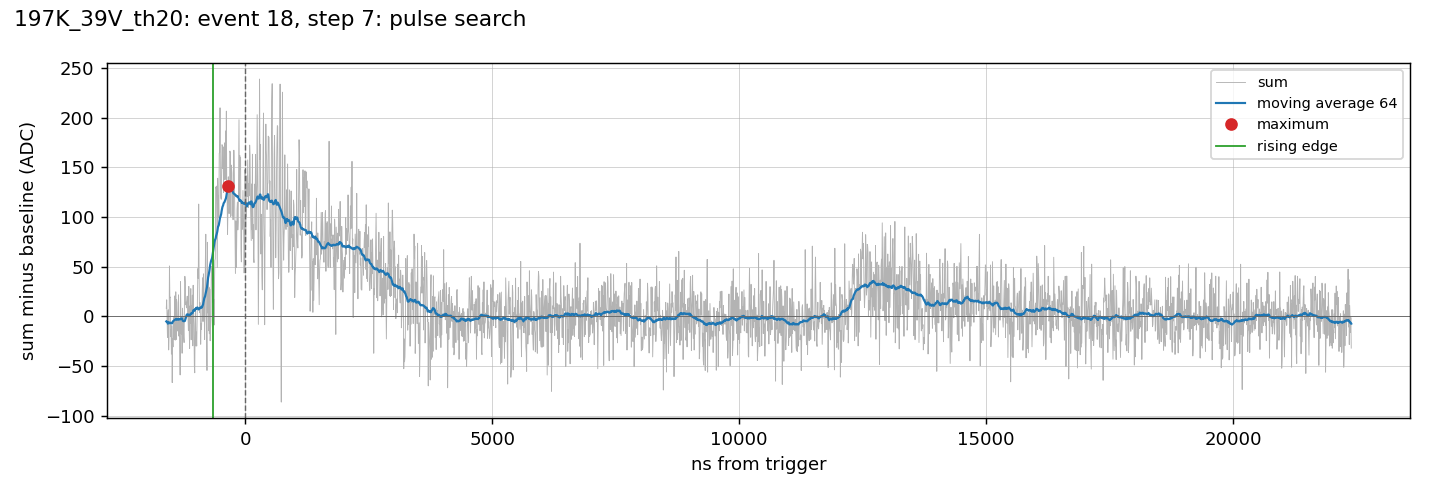
\includegraphics[width=\textwidth]{figs/sel_197K_ev18_s7_pileup.png}\end{center}

\section{Figures}

One figure per step (none for step~10), titled with the run, the event
and the step; step~12 redraws its figure for every threshold typed. With \code{--save NAME} they go to
\code{src/py/plots/NAME\_evE\_sN.png} with $E$ the event index and $N$
the step. The figures of this document are in \code{docs/figs/} (tracked
in git) and were made with
\begin{lstlisting}
python3 src/py/selection.py 197K_39V_th20 --events 1 --save walk
python3 src/py/selection.py 128K_37V_th19 --events 0 --save tail
python3 src/py/selection.py 197K_39V_th20 --events 18 --save pileup
\end{lstlisting}
and copied from \code{src/py/plots/} with the names used above.

\section{Examples}

\begin{lstlisting}
# walk through event 0 of the cold run
python3 src/py/selection.py 128K_37V_th19

# ten events of a low-bias run, no prompts, figures saved
python3 src/py/selection.py 197K_39V_th20 --events 0-9 --save 197K

# one event from the interpolation step on, with the unprotected median for comparison
python3 src/py/selection.py 185K_39d5V_th19 --events 7 --from-step 4 --cm median
\end{lstlisting}

\end{document}
